\chapter{Support Vector Machines}

\section{Discriminant Functions}
A discriminant is a function that takes an input vector $x$ and assigns it to one of $K$ classes, denoted $C_k$
The simplest representation of a linear discriminant function is obtained by taking a linear function of the input vector so that
\begin{equation}
    \label{eq: discriminant classifier}
    y(x) = w^Tx + w_0    
\end{equation}

where $w=(w_0, ..., w_{M-1})^T$ and $x=(x_1, ..., x_D)^T$. $w$ is called a weight vector, and $w_0$ is a bias. An input vector $x$ is assigned to class $C_1$ if $y(x) \geq 0$ and to class $C_2$ otherwise. The corresponding decision boundary is therefore defined by the relation $y(x)=0$, which corresponds to a $(D-1)$

Consider two points $x_A$ and $x_B$ both of which lie on the decision surface. Because $y(x_A) = y(x_B) = 0$, we have $w^T(x_A - x_B)=w^TA - w^TB=0$ and hence the vector $w$ is orthogonal to every vector lying within the decision surface.

If $x$ is a point on the decision surface, then $y(x) = 0$, then
\begin{equation}
    y(x) = 0 \Leftrightarrow w^Tx + w_0 = 0 \Leftrightarrow w^Tx = -w_0 \Leftrightarrow \frac{w^Tx}{||w||} = - \frac{w_0}{||w||}
\end{equation}

The bias parameter $w_0$ determines the location of the decision surface.
Consider an arbitrary point $x$ and let $x_\bot$ be its orthogonal projection onto the decision surface, so that
\begin{equation}
    x = x_\bot + r \frac{w}{||w||} \Leftrightarrow w^T x = w^Tx_\bot + r w^T \frac{w}{||w||} = w^Tx_\bot + r\frac{w^2}{||w||} = w^Tx_\bot + r||w||
\end{equation}

If we add $w_0$ to both sides of the above equation, we have
\begin{equation}
    w^T + x_0 = w^Tx_\bot + w_0 + r||w|| \Leftrightarrow y(x) = r||w|| \Leftrightarrow r = \frac{y(x)}{||w||}
\end{equation}

The value of $y(x)$ gives a signed measure of the perpendicular distance $r$ of the point $x$ from the decision surface. $r$ is called \textbf{perpendicular distance}.

\begin{figure}
    \centering
    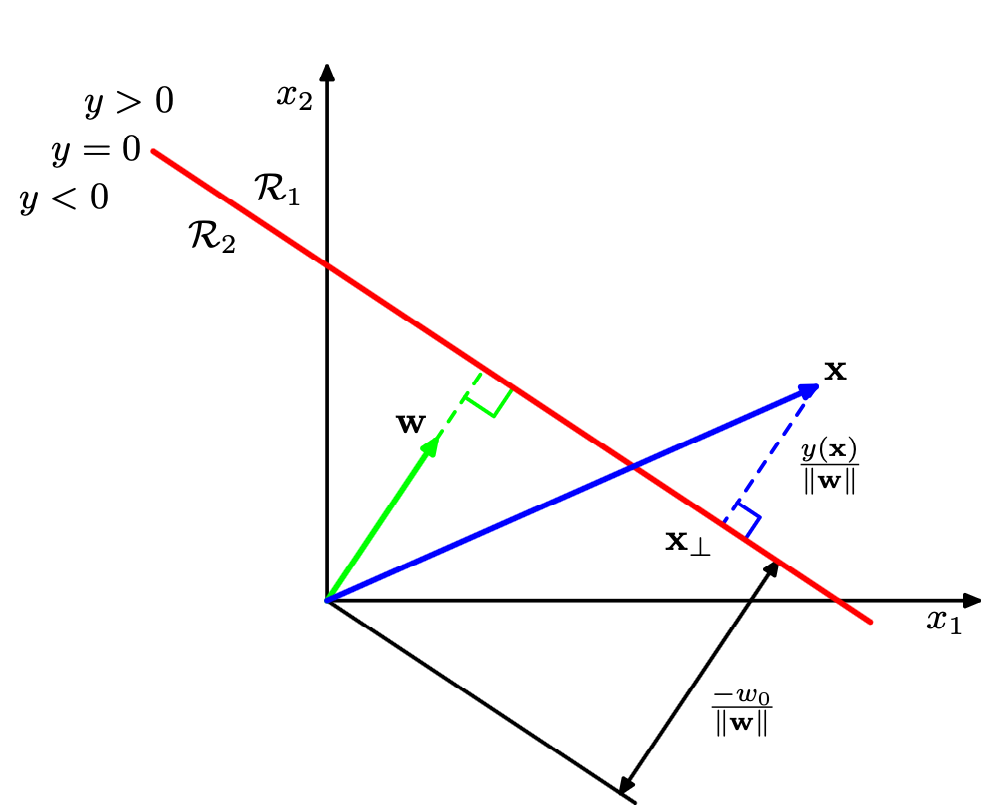
\includegraphics[scale=0.3]{chapter005/figures/fig003}
    \label{fig: geometry of a linear discriminant function}
    \caption{Illustration of the geometry of a linear discriminant function in two dimensions}
\end{figure}

\section{Maximum Margin Classifiers}

\begin{definition}
    Two-class classification problem using linear models of the form
    \begin{equation}
        \label{svm linear model}
        y(x)=w^T \phi (x) + b
    \end{equation}
    where $\phi (x)$ denotes a fixed feature-space transformation, and we have made the bias parameter $b$ explicit.
\end{definition}

The training data set comprises $N$ input vectors $x_1, ..., x_N$, with corresponding target values $t_1, ..., t_N$ where $t_n \in \{-1, 1\}$, and new data points $x$ are classified according to the sign of $y(x)$.

We shall assume for the moment that the training data set is linearly separable in feature space, so that by definition there exits at least one choice of the parameters $w$ and $b$ such that \ref{svm linear model} satisfies $y(x_n) > 0$ for points having $t_n = +1$ and $y(x_n) < 0$ for points having $t_n=-1$, so that $t_ny(x_n) > 0$ for all training data points.

The support vector machine minimize the generalization error through the concept of the $margin$, which is defined to be the smallest distance between the decision boundary and any of the samples.

\begin{figure}
    \centering
    \subfloat
        \centering
        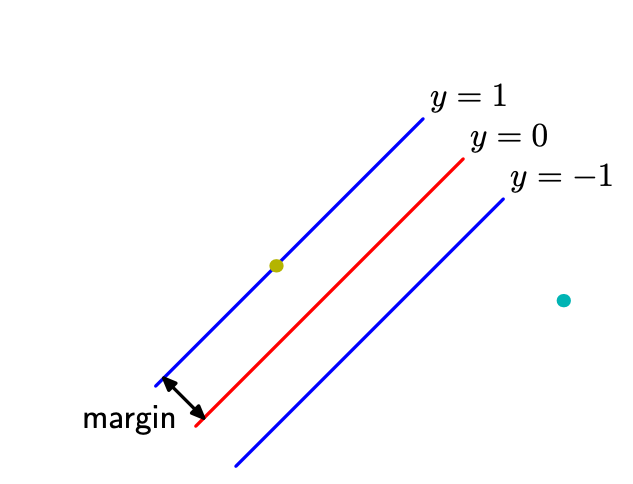
\includegraphics[width=5cm]{chapter005/figures/fig001}
    \qquad
    \subfloat
        \centering
            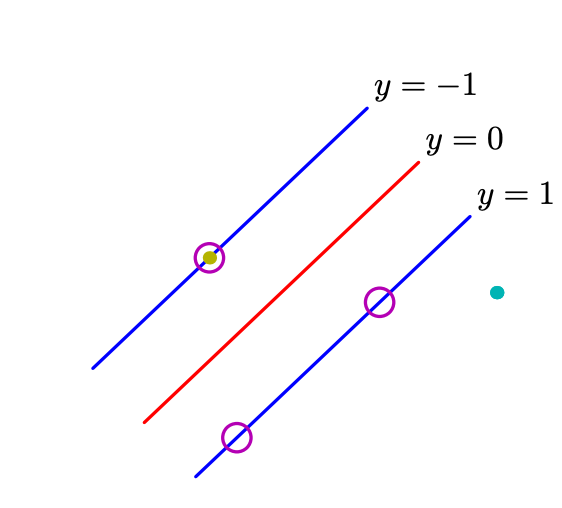
\includegraphics[width=5cm]{chapter005/figures/fig002}
    \label{fig:example}
    \caption{The margin is defined as the perpendicular distance between the decision boundary and the closest of the data points.}
\end{figure}

\textbf{In support vector machines, the decision boundary is chosen to be the one for which the margin is maximized}.

The perpendicular distance of a point $x$ from a hyperplane defined by $y(x)=0$ is given by $\frac{|y(x)|}{||w||}$.
We are only interested in solutions for which all data points are correctly classified, so that $t_ny(x_n)>0$ for all $n$.

Thus the distance of a point $x_n$ to the decision surface is given by
\begin{equation}
    \frac{t_ny(x_n)}{||w||} = \frac{t_n(w^T\phi(x_n) + b)}{||w||}
\end{equation}

The margin is given by the perpendicular distance to the closest point $x_n$ from the data set, and we wish to optimize the parameters $w$ and $b$ in order to maximum this distance. Thus the maximum margin solution is found by solving
\begin{align}
    \label{formula:SVM_optimize}
    \operatorname*{argmax}_{w,b} & \left \{ \frac{1}{||w||} \operatorname*{min}_{n}\left[ t_n(w^T\phi (x_n) + b) \right] \right \}
\end{align}

Note that if we make the rescaling $w \rightarrow kw$ and $b \rightarrow kb$, then the distance from any point $x_n$ to the decision surface, given by $t_ny(x_n)/||w||$, is unchanged.

\subsubsection{Proof}

Given $w=(w_0, ..., w_{M-1})$, then rescale $w \rightarrow kw$ means  $kw = (kw_0, ..., kw_{M-1})$, we have
\begin{equation}
    \label{eq: rescaling vector}
    \begin{split}
     ||kw|| & = \sqrt{(kw_0)^2 + (kw_1)^2 + ... + (kw_{M-1})^2} \\
            & = \sqrt{k^2(w_0^2 + w_1^2 + ... + w_{M-1}^2)} \\
            & = k||w||
     \end{split}
\end{equation}
and
\begin{equation}
       \frac{t_n((kw)^T\phi(x_n) + kb)}{||kw||}
        = \frac{kt_n((w)^T\phi(x_n) + b)}{k||w||} = \frac{t_n(w^T\phi(x_n) + b)}{||w||}
\end{equation}

We have,

\begin{equation}
    \frac{t_ny(x_n)}{||w||} = \frac{t_n(w^T\phi(x_n) + b)}{||w||} = d
\end{equation}

where $d$ is the distance from the closest data point to the hyper-plane. In other words,

\begin{equation}
    t_n(w^T\phi(x_n) + b) = d||w|| \Leftrightarrow \frac{t_n(w^T\phi(x_n) + b)}{d||w||} = 1
\end{equation}


\begin{align}
    \label{formula:SVM_optimize}
    \operatorname*{argmax}_{w,b} & \left \{ \frac{1}{||w||} \operatorname*{min}_{n}\left[ 1 \right] \right \} = \operatorname*{argmax}_{w,b}  \left \{ \frac{1}{||w||} \right \}
\end{align}

In this cases, all data points will satisfy the constraints

\begin{equation}
    \label{SVM: constraint}
    t_n(w^T\phi(x_n) + b) \geq 1, n =1,...,N
\end{equation}


The optimization problem then simply requires that we maximize $||w||^{-1}$, which is equivalent to minimizing $||w||^2$, and so we have to solve the optimization problem
\begin{equation}
    \operatorname*{arg\ min}_{w, b} \frac{1}{2}||w||^2
\end{equation}                                                                                                                                                                                     

subject to the constraints $t_n(w^T\phi(x_n) + b) \geq 1$. The factor of $\frac{1}{2}$ is included for later convenience.

Introduce Lagrangian function,
\begin{equation}
    L(w, b, a) = \frac{1}{2}||w||^2 - \sum_{n=1}^N a_n\{t_n(w^T \phi(x_n) + b) - 1 \}
\end{equation}

where $a = (a_1, ..., a_N)^T$ and $a_n \geq 0$ are Lagrange multipliers.

Setting the derivatives of $L(w, b, a)$ with respect to $w$ and $b$ equal to zero, we obtain the following

\begin{equation}
    \label{eq: w and a_n}
    \frac{\partial L(w, b, a)}{\partial w} = w - \sum_{n=1}^{N}a_n t_n \phi(x_n) = 0 \Leftrightarrow w = \sum_{n=1}^{N}a_n t_n\phi(x_n)
\end{equation}

and

\begin{equation}
    \frac{\partial L(w, b, a)}{\partial b} = \sum_{n=1}^{N}a_n t_n = 0 \Leftrightarrow \sum_{n=1}^{N}a_n t_n = 0
\end{equation}

Eliminating $w$ and $b$ from $L(w, b, a)$ using these conditions then gives 

\begin{equation}
    \begin{split}
    L(w, b, a) & = \frac{1}{2}||w||^2 - \sum_{n=1}^N a_n \{t_n(w^T \phi (x_n) + b) - 1\} \\
    & = \frac{1}{2}(\sum_{n=1}^{N} a_n t_n \phi (x_n) )^T(\sum_{n=1}^{N} a_n t_n \phi (x_n) ) - \sum_{n=1}^N a_n \{t_n(w^T \phi (x_n) + b) - 1\} \\
    & = \frac{1}{2}(\sum_{n=1}^{N} a_n t_n \phi (x_n)^T )(\sum_{n=1}^{N} a_n t_n \phi (x_n) ) - \sum_{n=1}^{N}a_n\{t_n w^T \phi(x_n) + t_n b - 1\} \\
    & = \frac{1}{2}(\sum_{n=1}^{N} a_n t_n \phi (x_n)^T )(\sum_{n=1}^{N} a_n t_n \phi (x_n) ) - \sum_{n=1}^{N}\{a_n t_n w^T \phi(x_n) + a_n t_n b - a_n\} \\
    & = \frac{1}{2}(\sum_{n=1}^{N} a_n t_n \phi (x_n)^T)(\sum_{n=1}^{N} a_n t_n \phi (x_n) ) - \sum_{n=1}^{N}a_n t_n w^T \phi(x_n) + \sum_{n=1}^{N}a_n t_n b + \sum_{n=1}^{N}a_n
    \end{split}
\end{equation}

Since $b$ is a just a number and $\sum_{n=1}^{N}a_n t_n = 0$, thus $\sum_{n=1}^{N}a_n t_n b = 0$. We have,

\begin{equation}
    \begin{split}
    L(w, b, a) & = \frac{1}{2}(\sum_{n=1}^{N} a_n t_n \phi (x_n)^T)(\sum_{n=1}^{N} a_n t_n \phi (x_n) ) - \sum_{n=1}^{N}a_n t_n w^T \phi(x_n) + \sum_{n=1}^{N}a_n t_n b + \sum_{n=1}^{N}a_n \\
    & = \frac{1}{2}(\sum_{n=1}^{N} a_n t_n \phi (x_n)^T)(\sum_{n=1}^{N} a_n t_n \phi (x_n) ) - \sum_{n=1}^{N}a_n t_n w^T \phi(x_n) + \sum_{n=1}^{N}a_n \\
    & = \frac{1}{2}(\sum_{n=1}^{N} a_n t_n \phi (x_n)^T)(\sum_{n=1}^{N} a_n t_n \phi (x_n)) - \sum_{n=1}^{N}a_n t_n (\sum_{n=1}^{N} a_n t_n \phi (x_n)^T) \phi(x_n) + \sum_{n=1}^{N}a_n \\
    & = -\frac{1}{2}\sum_{n=1}^{N}a_n t_n (\sum_{n=1}^{N} a_n t_n \phi (x_n)^T) \phi(x_n) + \sum_{n=1}^{N}a_n \\
    & = \sum_{n=1}^{N}a_n - \frac{1}{2}\sum_{n=1}^{N}\sum_{m=1}^{M} a_n a_m t_n t_m k (x_n, x_m)
    \end{split}
\end{equation}

Note that $a_n$ and $t_n$ are just numbers and $\phi(x_n)$ is a vector. Thus, $\sum_{n=1}^N a_nt_n\phi(x_n)^T$ and $\sum_{n=1}^N a_nt_n\phi(x_n)$ are summation of vectors which are also vectors and $k(x, x')=\phi(x)^T\phi(x')$

In order to classify new data points using the trained model, we evaluate the sign of $y(x)$ defined by \ref{eq: discriminant classifier}. This can be expressed in terms of the parameters $\{a_n\}$ and the kernel function by substituting for $w$ using \ref{eq: w and a_n} to give

\begin{equation}
    y(x) = \sum_{n=1}^{N} a_n t_n k(x, x_n) + b
\end{equation}

Recalling that the Lagrange function is defined by:

$$
    L(x, \lambda) \equiv f(x) + \lambda g(x)
$$

and we want to maximize $f(x)$ subject to a constraint relating $x_1$ and $x_2$, which we write in the form $g(x_1, x_2)=0$. 
Note that $\lambda$ can have either sign.

If we consider a problem of maximizing $f(x)$ subject to an inequality constraint of the form $g(x) \geq 0$. There are two kinds of solution possible

\begin{enumerate}
    \item if the constrained stationary point lies in the region where $g(x) > 0$, in which case the constrain is \textbf{inactive}. Because the point is far away the $f(x)$ function. At this moment, the function $g(x)$ plays no role and so the stationary condition is $\nabla f(x) = 0$ and the $\lambda = 0$. In other words, $\lambda g(x) = 0$
    \item if the point lies on the boundary $g(x) = 0$, in which case the constraint is \textbf{active}, then $\lambda \neq 0$. The function f(x) will only be at a maximum if its gradient is oriented way from the region $g(x) > 0$. Therefore, $\nabla f(x)$ and $\nabla g(x)$ are opposite to each other as illustrated in the below figure. For $\lambda > 0$, then $\nabla f(x) = - \lambda \nabla g(x)$. Because $g(x) = 0$, $\lambda g(x) = 0$.
\end{enumerate}
 
For either of these two cases, the product $\lambda g(x) = 0$. Thus the solution to the problem of maximizing $f(x)$ subject to $g(x) \geq 0$ is obtained by optimizing the Lagrange function with respect to $x$ and $\lambda$ subject to the conditions

\begin{equation}
  \left\{
    \begin{aligned}
      & g(x) \geq 0\\
      & \lambda \geq 0\\
      & \lambda g(x) = 0
    \end{aligned}
  \right.
\end{equation}
 
These are known as the \textbf{Karush-Kuhn-Tucker} (KKT) conditions.

In \textbf{SVM}, we have

\begin{equation}
  \left\{
    \begin{aligned}
      & a_n \geq 0\\
      & t_n y(x_n) - 1 \geq 0\\
      & a_n \{t_n y (x_n) - 1\} = 0
    \end{aligned}
  \right.
\end{equation}

The data points which caused $a_n = 0$ and satisfy $t_n y(x_n) = 1$ is called \textbf{Support Vectors}. They correspond to points that lie on the maximum margin hyperplanes in feature space. Once the model is trained, a significant proportion of the data points can be discarded and only the support vectors retained.

\begin{figure}
    \centering
    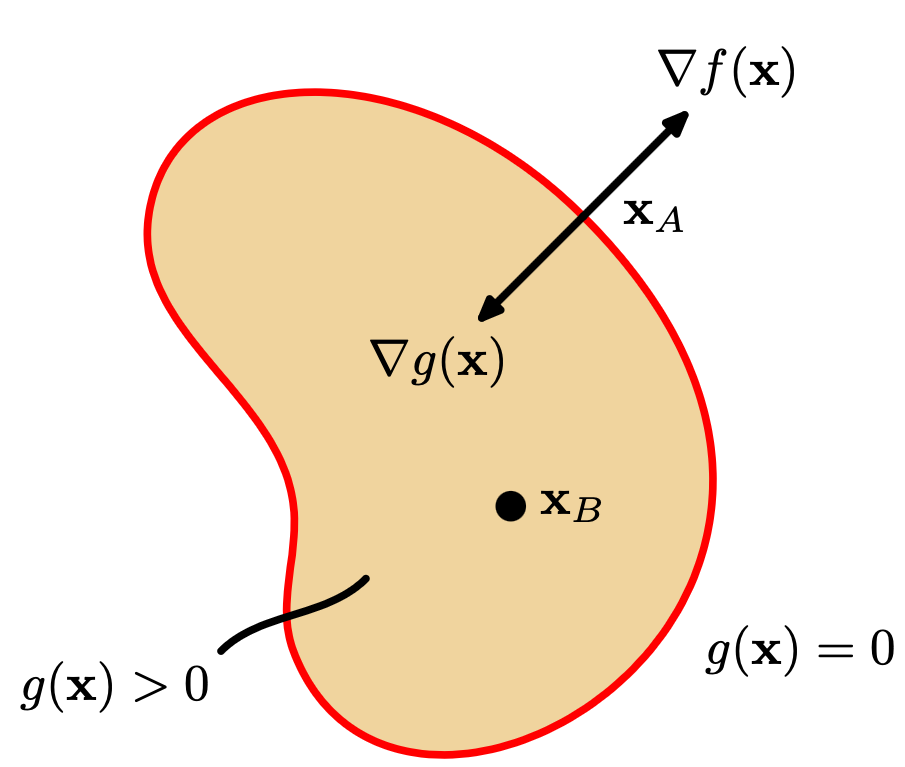
\includegraphics[width=5cm]{chapter005/figures/fig004}
    \caption{Lagrange Multipliers subject to $g(x) \geq 0$}
\end{figure}

Any support vector $x_n$ satisfies $t_ny(x_n)=1$, gives

\begin{equation}
    t_n (\sum_{m \in S} a_m t_m k(x_n, x_m) + b) = 1
\end{equation}

where $S$ denotes the set of indices of the support vectors.

\begin{equation}
    \begin{split}
    1 & = t_n (\sum_{m \in S} a_m t_m k(x_n, x_m) + b) \\
    & = t_n \sum_{m \in S} a_m t_m k(x_n, x_m) + t_nb \\
    \Leftrightarrow t_n & = t_n^2 \sum_{m \in S} a_m t_m k(x_n, x_m) + t_n^2b\\
    \Leftrightarrow t_n^2b & = t_n - t_n^2 \sum_{m \in S} a_m t_m k(x_n, x_m)\\
    \Leftrightarrow b & = t_n - \sum_{m \in S} a_m t_m k(x_n, x_m)\\
    \Leftrightarrow \sum_{n \in S} b & = \sum_{n \in S} (t_n - \sum_{m \in S} a_m t_m k(x_n, x_m))\\
    \Leftrightarrow N_S b & = \sum_{n \in S} (t_n - \sum_{m \in S} a_m t_m k(x_n, x_m))\\
    \Leftrightarrow b & = \frac{1}{N_S}\sum_{n \in S} (t_n - \sum_{m \in S} a_m t_m k(x_n, x_m))\\
    \end{split}
\end{equation}

where $N_S$ is the total number of support vectors.
Since $t_n=\pm 1$, $t_n^2=1$.

For later comparison with alternative models, we can express the maximum margin classifier in terms of the minimization of an error function, with a sample quadratic regularizer, in the form

\begin{equation}
    \label{form: svm error function}
    \sum_{n=1}^N E_\infty (y(x_n)t_n - 1) + \lambda ||w||^2
\end{equation}


Because the expected value of $y(x_n)t_n=1$, the \ref{form: svm error function} is minimum when $y(x_n)t_n=1$.

$E_\infty(z)$ is a function that is zero if $z \geq 0$ and $\infty$ otherwise and ensure that the constrain \ref{SVM: constraint} are satisfied.

 \section{Overlapping Class Distribution}
 
 We implicitly used an error function that gave infinite error if a data point was misclassified and zero error if it was classified correctly, and then optimized the model parameters to maximize the margin.
 
 We now modify this approach so that data points are allowed to be on the \textbf{wrong side} of the margin boundary, but with a penalty that increases with the distance from that boundary.
 
 To do this, we introduce \textbf{slack variables}, $\xi_n \geq 0$ where $n=1, ..., N$.
 
 These are defined by $\xi_n = 0$ for data points that are on or inside the correct margin boundary and $\xi_n = |t_n - y(x_n)|$ for other points. Thus a data point tht is on the decision boundary $y(x_n)=0$ will have $\xi_n=1$. $\xi_n > 1$ will be misclassified.
 
 The exact classification constraints are then replaced with
 \begin{equation}
    \label{SVM: slack variable constraint}
     t_ny(x_n) \geq 1 - \xi_n, n = 1,...,N
 \end{equation}
 in which the slack variables are constrained to satisfy $\xi \geq 0$. Data points for which $\xi \geq 0$ are correctly classified ($t_n = y(x_n)$). Points for which $0 < \xi \leq 1$ lie inside the margin, but on the correct side of the decision boundary. Those data points for which $\xi > 1$ lie on the wrong side of the decision boundary and are misclassified.
 
 
 \begin{figure}
    \centering
    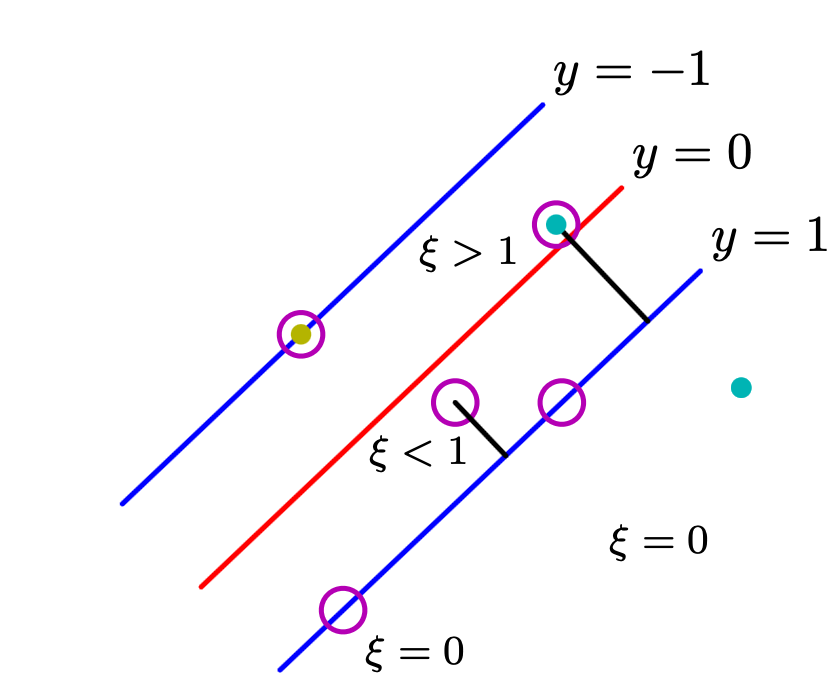
\includegraphics[width=5cm]{chapter005/figures/fig005}
    \caption{Illustration of the $\xi$ variable}
\end{figure}

This is sometimes described as relaxing the hard margin constraint to give a \textbf{soft margin} and allows some the training set data points to be misclassified.

Note that while slack variables allow for overlapping class distributions, this framework is still sensitive to outliers because the penalty for misclassification increases linearly with $\xi$.

Our goal is now to maximize the margin while softly penalizing points that lie on the wrong side of the margin boundary. We therefore minimize

\begin{equation}
    \label{SVM: C loss function}
    C \sum_{n=1}^N \xi_n + \frac{1}{2} ||w||^2
\end{equation}

where the parameter $C > 0$ controls the trade-off between the slack variable penalty and the margin. Because any point that is misclassified has $\xi > 1$, it follows that $\sum_n \xi_n$ is an upper bound on the number of misclassified points. The parameter $C$ is therefore analogous to a regularization coefficient because it controls the trade-off between minimizing training errors and controlling model complexity.

In the limit $C \rightarrow \infty$, we will recover the earlier support vector machine for separable data.

We now wish to minimize \ref{SVM: C loss function} subject to the constraints \ref{SVM: slack variable constraint} together with $\xi_n \geq 0$

The corresponding Lagrangian is given by

\begin{equation}
    \label{form: SVM Lagrangian}
    L(w, b, \xi, a, \mu) = \frac{1}{2} ||w||^2 + c\sum_{n=1}^N \xi_n - \sum_{n=1}^Na_n\{t_ny(x_n) - 1 + \xi_n\} - \sum_{n=1}^N \mu_n \xi_n
\end{equation}

Note that the constrain \ref{SVM: slack variable constraint} $\Leftrightarrow t_ny(x_n) - 1 + \xi_n \geq 0$
 
Where $\{a_n \geq 0\}$ and $\{\mu_n \geq 0 \}$ are Lagrange multipliers. The corresponding set of KKT conditions are given by


\begin{equation}
    \label{SVM: Lagrangian Soft-margin constraints}
  \left\{
    \begin{aligned}
      & a_n \geq 0\\
      & t_n y(x_n) - 1 + \xi_n \geq 0\\
      & a_n \{t_n y (x_n) - 1 + \xi_n \} = 0\\
      & \mu_n \geq 0\\
      & \xi_n \geq 0\\
      & \mu_n \xi_n = 0
    \end{aligned}
  \right.
\end{equation}

where $n=1,...,N$.

We know optimize out $w$, $b$ and $\{\xi_n\}$, then

\begin{equation}
    \frac{\partial L}{\partial w} = 0 \Leftrightarrow \frac{ \partial [\frac{1}{2} ||w||^2 - \sum_{n=1}^N a_n t_n w^T \phi(x_n) + \sum_{n=1}^N a_n t_n b - \sum_{n=1}^Na_n + \sum_{n=1}^Na_n \xi_n ]}{\partial w}= 0
\end{equation}

then,

\begin{equation}
    w - \sum_{n=1}^N a_n t_n \phi(x_n) = 0 \Leftrightarrow w = \sum_{n=1}^N a_n t_n \phi(x_n)
\end{equation}

In the similarity, we have

\begin{equation}
    \label{SVM: solution of Lagrange soft-margin}
  \left\{
    \begin{aligned}
      & \frac{\partial L}{\partial w} = 0 \Rightarrow \sum_{n=1}^N a_n t_n = 0\\
      & \frac{\partial L}{\partial \xi_n} = 0 \Leftrightarrow \sum_{n=1}^NC - \sum_{n=1}^Na_n - \sum_{n=1}^N \mu_n = 0 \Leftrightarrow  \sum_{n=1}^N(C - a_n - \mu_n) = 0 \Leftrightarrow a_n = C- \mu_n
    \end{aligned}
  \right.
\end{equation}

Then,

from \ref{form: SVM Lagrangian}, we have

\begin{equation}
    \label{SVM: Lagrange loss}
    L(a) = \sum_{n=1}^N a_n - \frac{1}{2}\sum_{n=1}^N\sum_{m=1}^N a_n a_m t_n t_m k(x_n, x_m)  
\end{equation}


which is identical to the separable case, except that the constraints are somewhat different. To see what these constraints are, we note that $a_n \geq 0$ is required because these are Lagrange multipliers.

Together with $u_n \geq 0$ implies $a_n \leq C$. We therefore have to maximize \ref{SVM:  Lagrange loss} with respect to the dual variables $\{a_n\}$ subject to

\begin{equation}
  \left\{
    \begin{aligned}
      & 0 \leq a_n \leq C\\
      & \sum_{n=1}^N a_n t_n = 0
    \end{aligned}
  \right.
\end{equation}

for $n=1, ..., N$.

\begin{enumerate}
    \item if $a_n = 0$, they do not contribute to the predictive model.
    \item if $a_n > 0$, from \ref{SVM: Lagrangian Soft-margin constraints}, we have $a_n(t_ny(x_n) -1 + \xi_n) = 0 \Leftrightarrow t_ny(x_n) -1 + \xi_n = 0$. Then, $t_ny(x_n) = 1 - \xi_n$.
    \item if $a_n < C$, then from \ref{SVM: solution of Lagrange soft-margin}, we have $a_n = C - \mu_n \Leftrightarrow \mu_n = C - a_n \Leftrightarrow \mu_n > 0$. From \ref{SVM: Lagrangian Soft-margin constraints}, we have $\mu_n \xi_n = 0$, thus $\xi_n = 0$. In other words, data points lie on the margin.
    \item if $a_n = C$, then $\mu_n = 0$. At this moment, we have 2 cases. If $\xi_n = 0$, then the points lie inside the margin. The last case is $\xi_n \neq 0$, it leads to 2 sub-cases. If $\xi_n \leq 1$, the points is correctly classified. Otherwise, they are misclassified.
\end{enumerate}


